%%
% Building some illustrations for later
%%
% \documentclass[aspectratio=169, 169]{beamer}
\documentclass{beamer}

\usepackage{algorithm}
\usepackage[noend]{algpseudocode}
\usepackage{array}
\usepackage{amsfonts}
\usepackage{amssymb}
\usepackage[T1]{fontenc}
\usepackage{fourier}
\usepackage[utf8]{inputenc}
\usepackage{minted}
\usepackage{stmaryrd}
\usepackage{subfig}
\usepackage{tikz}
\usepackage{verbatim}
\usepackage{xcolor}

\usepackage{algorithm}
\usepackage[noend]{algpseudocode}


% \usetheme{ENS}
% \usetheme{Singapore}
\usetheme[secheader]{Boadilla}
\usefonttheme[onlymath]{serif}

\usetikzlibrary{arrows}
\usetikzlibrary{decorations.pathreplacing}
\usetikzlibrary{math}
\usetikzlibrary{positioning}

\renewcommand{\thealgorithm}{}
\beamertemplatenavigationsymbolsempty

% Automaton setup
\usetikzlibrary{arrows.meta, automata, bending, positioning, shapes.misc}
\tikzstyle{automaton}=[shorten >=1pt, >={Stealth[bend,round]}, initial text=]

% Function symbols
\newcommand{\Span}[1]{\left[ #1 \right\rangle}

% Add blocks
\newenvironment{theoremblock}[1]{%
  \setbeamercolor{block body}{bg=black!3, fg=black}
  \setbeamercolor{block title}{bg=black!80, fg=white}
  \begin{block}{#1}}{\end{block}}

\title[M2 internship]{%
  Constant delay enumeration for documents spanners
}
\subtitle{M2 internship}
\author[Rémi Dupré]{%
  Rémi Dupré \\
  Supervised by Antoine Amarilli and Pierre Senellart
}
\institute[ENS / Télécom Paris]{ENS Paris / Télécom Paris}
\date{March --- August 2019}


% TODO: parler en regex partout

\begin{document}
\maketitle

\section{Introduction}

  \begin{frame}{Introduction}
    % Introduire un exemple
    % Introduire ce que j'ai fait

    \only<1>{%
      \[
        E = \underbrace{\texttt{AUG}}_{\hidewidth\text{exact
        text}\hidewidth}\overbrace{(...)\{0,2\}}^{\hidewidth \text{a text of
        size 3, 6 or 9}
        \hidewidth}\underbrace{\texttt{UAA}}_{\hidewidth\text{exact
        text}\hidewidth}
      \]
    }
    \onslide<2->{%
      \[
        E = \texttt{AUG}(...)\{0,2\}\texttt{UAA}
      \]
    }

    \only<1-3>{%
      \[
        w = \texttt{AUGAUGCGCUAAUAA}
      \]
    }
    \only<4>{%
      \[
        w = \texttt{\underline{AUGAUGCGCUAA}UAA}
      \]
    }
    \only<5>{%
      \[
        w = \texttt{AUG\underline{AUGCGCUAA}UAA}
      \]
    }
    \only<6>{%
      \[
        w = \texttt{AUG\underline{AUGCGCUAAUAA}}
      \]
    }

    \vspace{\fill}
    \null
    \vfill

    \begin{itemize}
      \item<2-> does $w$ match $E$?
      \item<3-> is there a factor of $w$ matching $E$?
      \item<4-> what are all the factors of $w$ matching $E$?
    \end{itemize}

  \end{frame}

  % \begin{frame}{Automata (1)}
  %   \begin{block}{Definition: Automaton}
  %     A \textit{finite automaton} $\mathcal{A}$ over a finite alphabet
  %     $\Sigma$ is a tuple $(Q, q_\text{init}, \Delta, F)$ where:
  %     \begin{itemize}
  %       \item $Q$ is the finite set of states;
  %       \item $q_\text{init} \in Q$ is the initial states;
  %       \item $F \subseteq Q$ is the set of final states;
  %       \item $\Delta \subseteq Q \times \Sigma \times Q$ is the transition
  %         function.
  %     \end{itemize}
  %   \end{block}
  %
  %   \begin{figure}[ht]
  %     \centering
  %     \begin{tikzpicture}[automaton, auto]
  %       \node[state,initial]   (1)              {$q_0$};
  %       \node[state]           (3) [right=of 1] {$q_1$};
  %       \node[state]           (4) [right=of 3] {$q_2$};
  %       \node[state,accepting] (6) [right=of 4] {$q_3$};
  %
  %       \path[->]
  %         (1) edge node {$\Sigma \setminus \texttt \textvisiblespace$} (3)
  %             edge [loop above] node {$\Sigma$} ()
  %         (3) edge node {$@$} (4)
  %             edge [loop above] node {$\Sigma \setminus \texttt
  %             \textvisiblespace$} ()
  %         (4) edge node {$\Sigma \setminus \texttt \textvisiblespace$} (6)
  %             edge [loop above] node {$\Sigma \setminus \texttt
  %             \textvisiblespace$} ()
  %         (6) edge [loop above] node {$\Sigma$} ();
  %     \end{tikzpicture}
  %     \caption{%
  %       An automaton recognising simplified email patterns
  %     }%
  %     \label{fig:automata_simple}
  %   \end{figure}
  % \end{frame}

  % \begin{frame}{Automata (2)}
  %   \onslide<2->{%
  %     \begin{alertblock}{Problem: Membership}
  %       Given an automaton $\mathcal{A}$ and a word $w \in \Sigma^*$, test if
  %       $w \in L(\mathcal{A})$ where $L(\mathcal{A})$ is the language of
  %       words accepted by $\mathcal{A}$.
  %     \end{alertblock}
  %   }
  %
  %   \onslide<3->{
  %     \begin{algorithm}[H]%
  %       \begin{algorithmic}[1]
  %         \State{$S \gets \{q_{\text{init}}\}$}
  %         \For{$i = 0$ to $|w|$}
  %           \State{%
  %             $S \gets \{q' \mid \exists q \in S, (q, w_i, q') \in \Delta\}$}
  %         \EndFor{}
  %         \State{\Return{$S \cap F \neq \emptyset$}}
  %       \end{algorithmic}
  %       \caption{%
  %         Testing $w \in L(\mathcal{A})$ in time $O(|w| \cdot |\mathcal{A}|)$}
  %     \end{algorithm}
  %   }
  % \end{frame}

\section{Problem Setup}

  \begin{frame}{The problem of enumeration}
    \begin{alertblock}{Problem 1: Weak}
      Given a regular expression $E$ and a word $w \in \Sigma^*$, output all
      the pairs $(i, j)$ such that $w_i \ldots w_j \in L(E)$.
    \end{alertblock}

    \begin{itemize}
      \onslide<2->{\item very naïve: $O(|w|^3)$}
      \onslide<3->{\item still simple: $O(|w|^2)$}
    \end{itemize}

    \onslide<4->{\danger{} output can be of size $O(|w|^2)$}

    \vspace{-1mm}

    \only<2>{%
      \begin{algorithm}[H]%
        \begin{algorithmic}[1]
          \State{$S \gets \{q_{\text{init}}\}$}
          \For{$i = 0$ to $|w|$}
            \State{%
              $S \gets \{q' \mid \exists q \in S, (q, w_i, q') \in \Delta\}$}
          \EndFor{}
          \State{\Return{$S \cap F \neq \emptyset$}}
        \end{algorithmic}
        \caption{%
          Testing $w \in L(\mathcal{A})$ in time $O(|w| \cdot |\mathcal{A}|)$}
      \end{algorithm}
    }

    \onslide<3->{%
      \begin{algorithm}[H]%
        \begin{algorithmic}[1]
          \State{$\texttt{output} \gets \emptyset$}
          \For{$i = 0$ to $|d|$}
            \State{$S \gets \{q_\text{init}\}$}
            \For{$j = i$ to $|d|$}
              \If{$S \cap F \neq \emptyset$}
                \State{%
                  $\texttt{output} \gets \texttt{output} \uplus \{(i,
                  j)\}$
                }
              \EndIf{}
              \State{%
                $S \gets \{q' \in Q, \exists q \in S, (q, d_j, q') \in \Delta
                \}$
              }
            \EndFor{}
          \EndFor{}
        \end{algorithmic}
        \caption{%
          Enumerate all matching factors in time $O(|w|^2 \cdot
          \mathcal{|A|})$
        }
      \end{algorithm}
    }
  \end{frame}

  \begin{frame}{Enumeration complexity}
    Idea: split the algorithm in two parts:
      \begin{itemize}
        \item a preprocessing phase
        \item an enumeration phase with a constant delay
          in-between delay
      \end{itemize}

    \vspace{1cm}

    \onslide<2->{%
      \begin{theoremblock}{Theorem (2019): Amarilli, Bourhis, Mengel, Niewerth}
        This can be done with preprocessing time in $O((|Q|^4 + |\mathcal{A}|)
        \times |d|)$ and with delay $O(|Q|^2 + |\mathcal{A}|$).
      \end{theoremblock}
    }
  \end{frame}

  \begin{frame}{Document spanners}
    \Large
    A \emph{document}:
    \only<-1>{
      \Large \[
        d = d_1 d_2 \ldots d_n
        \qquad \left(\in \Sigma^*\right)
      \]
    }
    \only<2->{
      \Large \[
        d = d_1 d_2 \ldots \underbrace{d_i \ldots d_{j-1}}_{\text{a
        \emph{span} } \Span{i, j}} \ldots d_n
        \qquad \left(\in \Sigma^*\right)
      \]
    }

    \onslide<3->{
      A finite set of \emph{variables}:
      \[
        \mathcal{V} = \{ x, y \ldots \}
      \]
    }

    \vspace{-5mm}

    \onslide<4->{
      A \emph{document spanner} ouput a set of \emph{results} in the form:

      \begin{columns}
        \begin{column}{0.25\textwidth}
          \[
            \begin{cases}
              x \mapsto \Span{i_x, j_x} \\
              y \mapsto \Span{i_y, j_y} \\
              \cdots
            \end{cases}
          \]
        \end{column}
        \begin{column}{0.65\textwidth}
          \[
            d_1 \ldots \overbrace{d_{i_x} \ldots d_{j_x - 1}}^{x} \ldots
            \underbrace{d_{i_y} \ldots d_{j_y
            - 1}}_{y} \ldots d_n
          \]
          % i.e.\ partials mappings from $\mathcal{V}$ to spans of $d$
        \end{column}
      \end{columns}

      \[
        % r = \left\{
        %   m_2: \begin{cases}
        %     x \mapsto \Span{i_{x, 1}, j_{x, 1}}
        %   \end{cases}
        %   \cdots
        % \right\}
      \]
    }

  \end{frame}

  % \begin{frame}{Document spanners}
  %   \begin{block}{Vocabulary}
  %     \begin{itemize}
  %       \item a word $d \in \Sigma^*$ is called a \emph{document}
  %       \item a factor $d_i \ldots d_{j-1}$ is represented by a \emph{span}
  %         $\Span{i, j}$
  %       \item $\mathcal{V}$ is a finite set of \emph{variables}
  %       \item a \emph{result} is a partial mapping from $\mathcal{V}$ to spans
  %         of $d$
  %     \end{itemize}
  %   \end{block}
  %
  %   \onslide<2->
  %   \begin{block}{Definition: document spanner}
  %     A \emph{document spanner} over a finite set $\mathcal{V}$ of variables is
  %     a function defined on documents, which maps every document $d$ to sets of
  %     results over $\mathcal{V}$ on $d$.
  %   \end{block}
  %
  %   \onslide<3->
  %   \begin{exampleblock}{Example}
  %     With $\mathcal{V} = \{x, y\}$, map the first column to $x$ and the second
  %     column to $y$ for each line of a CSV document.
  %   \end{exampleblock}
  % \end{frame}

  \begin{frame}{Regex formula}
    \begin{center}
      \[
        \underbrace{x\{\texttt{AUG}(...)\{0,2\} \texttt{UAA}\}}_{\text{assigned
        to $x$}}
        \ (...)\{0,100\}
        \ \underbrace{y\{\texttt{AUG}(...)\{0,2\}
        \texttt{UAA}\}}_{\text{assigned to $y$}}
      \]
      % \Large \[ \cdots x\{E_1\} \ E_2 \ y\{E_3\} \cdots \]
    \end{center}

    % \begin{block}{Definition: Variable markers}
    %   For any $x \in \mathcal{V}$, define:
    %     \begin{itemize}
    %       \item an \textit{open marker} $x{\vdash}$;
    %       \item a \textit{close marker} ${\dashv}x$.
    %     \end{itemize}
    %
    %   $\Gamma_\mathcal{V} = \{x{\vdash}, x \in \mathcal{V}\} \uplus
    %   \{{\dashv}x, x \in \mathcal{V}\}$
    % \end{block}

    \onslide<2->
    \begin{block}{Definition: Variable set automata}
      A \emph{variable automaton} (VA) $\mathcal{A}$ over a finite alphabet
      $\Sigma$ is a tuple $(Q, q_\text{init}, \Delta, F)$ where $q_\text{init}
      \in Q, F \subseteq Q \text{ and } \Delta \subseteq Q \times (\Sigma \uplus
      \Gamma_\mathcal{V}) \times Q$.

      $$\Gamma_\mathcal{V} = \{x{\vdash}, x \in \mathcal{V}\} \uplus
      \{{\dashv}x, x \in \mathcal{V}\}$$
    \end{block}

    \begin{figure}[ht]%
      \centering
      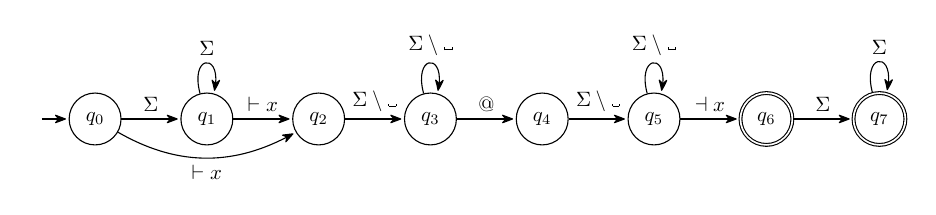
\begin{tikzpicture}[automaton, auto, scale=0.75, transform shape]
        \node[state,initial]   (0)              {$q_0$};
        \node[state]           (1) [right=of 0] {$q_1$};
        \node[state]           (2) [right=of 1] {$q_2$};
        \node[state]           (3) [right=of 2] {$q_3$};
        \node[state]           (4) [right=of 3] {$q_4$};
        \node[state]           (5) [right=of 4] {$q_5$};
        \node[state,accepting] (6) [right=of 5] {$q_6$};
        \node[state,accepting] (7) [right=of 6] {$q_7$};

        \path[->]
          (0) edge node {$\Sigma$} (1)
              edge [bend right] node [below] {$\vdash x$} (2)
          (1) edge node {$\vdash x$} (2)
              edge [loop above] node {$\Sigma$} ()
          (2) edge node {$\Sigma \setminus \texttt \textvisiblespace$} (3)
          (3) edge node {$@$} (4)
              edge [loop above] node {$\Sigma \setminus \texttt
              \textvisiblespace$} ()
          (4) edge node {$\Sigma \setminus \texttt \textvisiblespace$} (5)
          (5) edge node {$\dashv x$} (6)
              edge [loop above] node {$\Sigma \setminus \texttt
              \textvisiblespace$} ()
          (6) edge node {$\Sigma$} (7)
          (7) edge [loop above] node {$\Sigma$} ();
      \end{tikzpicture}
      % \caption{A variable automaton assigning email patterns to $x$}
    \end{figure}
  \end{frame}

  \begin{frame}{Enumeration for VAs}
    \begin{alertblock}{Problem 2: Strong}
      Given a regex formula $E$ and a document $d$, enumerate
      all the \textbf{distinct} \emph{results} defined by $E$ on $d$.
    \end{alertblock}


    \begin{theoremblock}{Theorem: Amarilli \& al., 2019}
      This can be done with preprocessing time in $O((|Q|^4 + |\mathcal{A}|)
      \times |d|)$ and with delay $O(|\mathcal{V}| \times (|Q|^2 +
      |\mathcal{A}| \times |\mathcal{V}|^2))$.
    \end{theoremblock}

    \vfill

    \onslide<2->{
      Reduction of the weak problem:
        \Large \[ E' = .* x\{E\} .* \]
      }
  \end{frame}

  % TODO: add a slide explaining runs for such an automaton

\section{Enumeration Algorithm}

  \begin{frame}{Product DAG}
    $d = \texttt{a@aa}$

    \begin{center}
      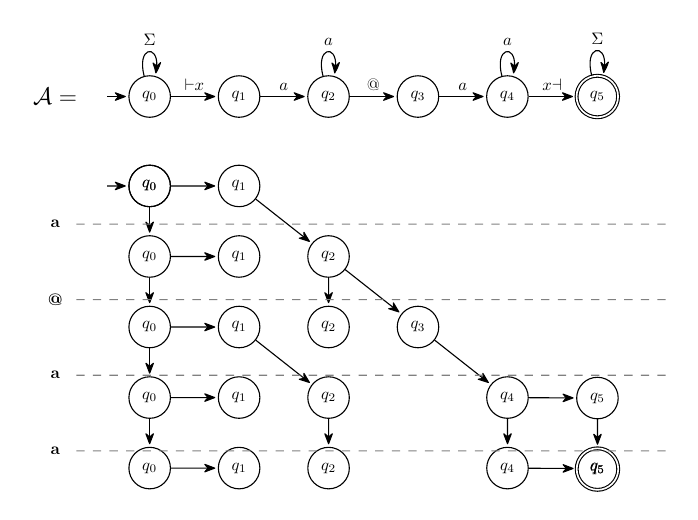
\begin{tikzpicture}[automaton, auto, scale=0.6, transform shape]
        % ==== AUTOMATON ====
        \node at (-2, 0) {\Large $\mathcal{A} = $};

        \node[state,initial]   (0)              {$q_0$};
        \node[state]           (1) [right=of 0] {$q_1$};
        \node[state]           (2) [right=of 1] {$q_2$};
        \node[state]           (3) [right=of 2] {$q_3$};
        \node[state]           (4) [right=of 3] {$q_4$};
        \node[state,accepting] (5) [right=of 4] {$q_5$};

        \path[->]
          (0) edge [loop above] node {$\Sigma$} ()
              edge node {${\vdash}x$} (1)
          (1) edge node {$a$} (2)
          (2) edge [loop above] node {$a$} ()
              edge node {$@$} (3)
          (3) edge node {$a$} (4)
          (4) edge node {$x{\dashv}$} (5)
              edge [loop above] node {$a$} ()
          (5) edge [loop above] node {$\Sigma$} ();

        % ==== DAG ====

        \onslide<2->{
          \node[state,draw=none] (02) [below=of 2] {};
          \node[state,draw=none] (03) [below=of 3] {};
          \node[state,draw=none] (04) [below=of 4] {};
          \node[state,draw=none] (05) [below=of 5] {};
        }
        \onslide<2-8>{
          \node[state]           (00) [below=of 0] {$q_0$};
        }
        \onslide<9->{
          \node[state,initial]   (00) [below=of 0] {$q_0$};
        }

        \onslide<3->{
          \node[state]           (01) [below=of 1] {$q_1$};
          \path[->]
            (00) edge (01);
        }

        \onslide<4->{
          \node[state]           (10) [below=6mm of 00] {$q_0$};
          \node[state]           (12) [below=6mm of 02] {$q_2$};
          \node[state,draw=none] (13) [below=6mm of 03] {};
          \node[state,draw=none] (14) [below=6mm of 04] {};
          \node[state,draw=none] (15) [below=6mm of 05] {};

          \path[->]
            (00) edge (10)
            (01) edge (12);
        }

        \onslide<5->{
          \node[state]           (11) [below=6mm of 01] {$q_1$};

          \path[->]
            (10) edge (11);
        }

        \onslide<6->{
          \node[state]           (20) [below=6mm of 10] {$q_0$};
          \node[state]           (21) [below=6mm of 11] {$q_1$};
          \node[state]           (22) [below=6mm of 12] {$q_2$};
          \node[state]           (23) [below=6mm of 13] {$q_3$};
          \node[state,draw=none] (24) [below=6mm of 14] {};
          \node[state,draw=none] (25) [below=6mm of 15] {};

          \path[->]
            (10) edge (20)
            (12) edge (22)
            (12) edge (23)
            (20) edge (21);
        }

        \onslide<7->{
          \node[state]           (30) [below=6mm of 20] {$q_0$};
          \node[state]           (31) [below=6mm of 21] {$q_1$};
          \node[state]           (32) [below=6mm of 22] {$q_2$};
          \node[state,draw=none] (33) [below=6mm of 23] {};
          \node[state]           (34) [below=6mm of 24] {$q_4$};
          \node[state]           (35) [below=6mm of 25] {$q_5$};

          \path[->]
            (20) edge (30)
            (21) edge (32)
            (23) edge (34)
            (30) edge (31)
            (34) edge (35);
        }

        \onslide<8->{
          \node[state]           (40) [below=6mm of 30] {$q_0$};
          \node[state]           (41) [below=6mm of 31] {$q_1$};
          \node[state]           (42) [below=6mm of 32] {$q_2$};
          \node[state,draw=none] (43) [below=6mm of 33] {};
          \node[state]           (44) [below=6mm of 34] {$q_4$};
          \node[state]           (45) [below=6mm of 35] {$q_5$};

          \path[->]
            (30) edge (40)
            (32) edge (42)
            (34) edge (44)
            (40) edge (41)
            (35) edge (45)
            (44) edge (45);
        }
        \onslide<8>{
          \node[state] (45)           [below=6mm of 35] {$q_5$};
        }
        \onslide<9->{
          \node[state,accepting] (45) [below=6mm of 35] {$q_5$};
        }

        % ==== WORD ====
        \onslide<4->{
          \node[state,draw=none] (w0)  at (-2, -2.7) {\textbf a};
          \path[-] (w0) edge [dashed, gray] (11, -2.7);
        }

        \onslide<6->{
          \node[state,draw=none] (w1) at (-2, -4.3) {\textbf @};
          \path[-] (w1) edge [dashed, gray] (11, -4.3);
        }

        \onslide<7->{
          \node[state,draw=none] (w2) at (-2, -5.9) {\textbf a};
          \path[-] (w2) edge [dashed, gray] (11, -5.9);
        }

        \onslide<8->{
          \node[state,draw=none] (w3) at (-2, -7.5) {\textbf a};
          \path[-] (w3) edge [dashed, gray] (11, -7.5);
        }
      \end{tikzpicture}
    \end{center}

    \onslide<9->

    \begin{itemize}
      \item two results: $x \mapsto \Span{0, 3}$ and $x \mapsto \Span{0, 4}$
    \end{itemize}
  \end{frame}

  \begin{frame}{Running over the DAG}
    \begin{itemize}
      \item several paths can anotate the same result
      \item naïve linear delay
    \end{itemize}

    \begin{center}
      \begin{tikzpicture}[automaton, auto, scale=0.6, transform shape]
        % ==== DAG ====

          \node[state,draw=none] (02) [below=of 2] {};
          \node[state,draw=none] (03) [below=of 3] {};
          \node[state,draw=none] (04) [below=of 4] {};
          \node[state,draw=none] (05) [below=of 5] {};
          \node[state,initial]   (00) [below=of 0] {$q_0$};

          \node[state]           (01) [below=of 1] {$q_1$};
          \path[->]
            (00) edge (01);

          \node[state]           (10) [below=6mm of 00] {$q_0$};
          \node[state]           (12) [below=6mm of 02] {$q_2$};
          \node[state,draw=none] (13) [below=6mm of 03] {};
          \node[state,draw=none] (14) [below=6mm of 04] {};
          \node[state,draw=none] (15) [below=6mm of 05] {};

          \path[->]
            (00) edge (10)
            (01) edge (12);

          \node[state]           (11) [below=6mm of 01] {$q_1$};

          \path[->]
            (10) edge (11);

          \node[state]           (20) [below=6mm of 10] {$q_0$};
          \node[state]           (21) [below=6mm of 11] {$q_1$};
          \node[state]           (22) [below=6mm of 12] {$q_2$};
          \node[state]           (23) [below=6mm of 13] {$q_3$};
          \node[state,draw=none] (24) [below=6mm of 14] {};
          \node[state,draw=none] (25) [below=6mm of 15] {};

          \path[->]
            (10) edge (20)
            (12) edge (22)
            (12) edge (23)
            (20) edge (21);

          \node[state]           (30) [below=6mm of 20] {$q_0$};
          \node[state]           (31) [below=6mm of 21] {$q_1$};
          \node[state]           (32) [below=6mm of 22] {$q_2$};
          \node[state,draw=none] (33) [below=6mm of 23] {};
          \node[state]           (34) [below=6mm of 24] {$q_4$};
          \node[state]           (35) [below=6mm of 25] {$q_5$};

          \path[->]
            (20) edge (30)
            (21) edge (32)
            (23) edge (34)
            (30) edge (31)
            (34) edge (35);

          \node[state]           (40) [below=6mm of 30] {$q_0$};
          \node[state]           (41) [below=6mm of 31] {$q_1$};
          \node[state] (42) [below=6mm of 32] {$q_2$};
          \node[state,draw=none] (43) [below=6mm of 33] {};
          \node[state]           (44) [below=6mm of 34] {$q_4$};
          \node[state]           (45) [below=6mm of 35] {$q_5$};

          \path[->]
            (30) edge (40)
            (32) edge (42)
            (34) edge (44)
            (40) edge (41)
            (35) edge (45)
            (44) edge (45);
          \node[state,accepting] (45) [below=6mm of 35] {$q_5$};

        % ==== WORD ====
        \node[state,draw=none] (w0)  at (-2, -2.7) {\textbf a};
        \path[-] (w0) edge [dashed, gray] (11, -2.7);

        \node[state,draw=none] (w1) at (-2, -4.3) {\textbf @};
        \path[-] (w1) edge [dashed, gray] (11, -4.3);

        \node[state,draw=none] (w2) at (-2, -5.9) {\textbf a};
        \path[-] (w2) edge [dashed, gray] (11, -5.9);

        \node[state,draw=none] (w3) at (-2, -7.5) {\textbf a};
        \path[-] (w3) edge [dashed, gray] (11, -7.5);

        % ==== RECTANGLES ====

        \onslide<2>
          \draw[draw=red] (9.15, -9) rectangle ++(1.5, 1.5);
        \onslide<3>
          \draw[draw=red] (9.15, -7.5) rectangle ++(1.5, 1.5);
        \onslide<4>
          \draw[draw=red] (7.15, -7.5) rectangle ++(1.5, 1.5);
        \onslide<5>
          \draw[draw=red] (1.2, -2.75) rectangle ++(1.5, 1.5);
        \onslide<6>
          \draw[draw=red] (-0.8, -2.75) rectangle ++(1.5, 1.5);

      \end{tikzpicture}

      \large \[
        \onslide<4->{x{\vdash}: 3}
        \onslide<6->{, {\dashv}x: 0}
      \]
    \end{center}
  \end{frame}

  \begin{frame}{Towards memory efficiency}
    \begin{itemize}
      \item $O(|Q| \times |d|)$ is way too much memory!
      \begin{itemize}
        \item<2-> only marker transitions have to be kept
        \item<3-> the index can actually be computed in streaming
      \end{itemize}
    \end{itemize}

    \vfill

    \begin{center}
      \begin{tikzpicture}[automaton, auto, scale=0.6, transform shape]
        % ==== DAG ====

          \node[state,draw=none] (02) [below=of 2] {};
          \node[state,draw=none] (03) [below=of 3] {};
          \node[state,draw=none] (04) [below=of 4] {};
          \node[state,draw=none] (05) [below=of 5] {};
          \node[state,initial]   (00) [below=of 0] {$q_0$};

          \node[state]           (01) [below=of 1] {$q_1$};
          \path[->]
            (00) edge (01);

          \onslide<1,2>{\node[state]           (10) [below=6mm of 00] {$q_0$};}
          \onslide<1>{\node[state]           (12) [below=6mm of 02] {$q_2$};}
          \node[state,draw=none] (13) [below=6mm of 03] {};
          \node[state,draw=none] (14) [below=6mm of 04] {};
          \node[state,draw=none] (15) [below=6mm of 05] {};

          \onslide<1>{
            \path[->]
              (00) edge (10)
              (01) edge (12);
          }

          \onslide<1,2>{\node[state]           (11) [below=6mm of 01] {$q_1$};}


          \onslide<1,2>{
            \path[->]
              (10) edge (11);
          }

          \onslide<1,2>{\node[state]           (20) [below=6mm of 10] {$q_0$};}
          \onslide<1,2>{\node[state]           (21) [below=6mm of 11] {$q_1$};}
          \onslide<1>{\node[state]           (22) [below=6mm of 12] {$q_2$};}
          \onslide<1>{\node[state]           (23) [below=6mm of 13] {$q_3$};}
          \node[state,draw=none] (24) [below=6mm of 14] {};
          \node[state,draw=none] (25) [below=6mm of 15] {};

          \onslide<1>{
            \path[->]
              (10) edge (20)
              (12) edge (22)
              (12) edge (23);
          }

          \onslide<1,2>{
            \path[->]
              (20) edge (21);
          }

          \onslide<1,2>{\node[state]           (30) [below=6mm of 20] {$q_0$};}
          \onslide<1,2>{\node[state]           (31) [below=6mm of 21] {$q_1$};}
         \onslide<1>{ \node[state]           (32) [below=6mm of 22] {$q_2$};}
          \node[state,draw=none] (33) [below=6mm of 23] {};
          \node[state]           (34) [below=6mm of 24] {$q_4$};
          \node[state]           (35) [below=6mm of 25] {$q_5$};

          \onslide<1>{
            \path[->]
              (20) edge (30)
              (21) edge (32)
              (23) edge (34);
            }
          \path[->]
            (34) edge (35);

          \onslide<1,2>{
          \path[->]
            (30) edge (31);
          }

          \onslide<1,2>{\node[state]           (40) [below=6mm of 30] {$q_0$};}
          \onslide<1,2>{\node[state]           (41) [below=6mm of 31] {$q_1$};}
          \onslide<1>{\node[state]           (42) [below=6mm of 32] {$q_2$};}
          \node[state,draw=none] (43) [below=6mm of 33] {};
          \node[state]           (44) [below=6mm of 34] {$q_4$};
          \node[state]           (45) [below=6mm of 35] {$q_5$};

          \onslide<1>{
            \path[->]
              (30) edge (40)
              (32) edge (42)
              (34) edge (44)
              (35) edge (45);
          }

          \onslide<1,2>{
            \path[->]
              (40) edge (41);
          }

          \path[->]
            (44) edge (45);
          \node[state,accepting] (45) [below=6mm of 35] {$q_5$};

          \onslide<2->{\path[->] (01) edge [gray] (34);}
          \onslide<2->{\path[->] (34) edge [gray] (44);}
          \onslide<2->{\path[->] (35) edge [gray] (45);}
          \onslide<2>{\path[->] (00) edge [gray] (10);}
          \onslide<2>{\path[->] (10) edge [gray] (20);}
          \onslide<2>{\path[->] (20) edge [gray] (30);}
          \onslide<2>{\path[->] (30) edge [gray] (40);}

        % ==== WORD ====
        \node[state,draw=none] (w0)  at (-2, -2.7) {\textbf a};
        \path[-] (w0) edge [dashed, gray] (11, -2.7);

        \node[state,draw=none] (w1) at (-2, -4.3) {\textbf @};
        \path[-] (w1) edge [dashed, gray] (11, -4.3);

        \node[state,draw=none] (w2) at (-2, -5.9) {\textbf a};
        \path[-] (w2) edge [dashed, gray] (11, -5.9);

        \node[state,draw=none] (w3) at (-2, -7.5) {\textbf a};
        \path[-] (w3) edge [dashed, gray] (11, -7.5);
      \end{tikzpicture}
    \end{center}

    \onslide<2>{}
  \end{frame}

  % \begin{frame}{Product DAG}
  %   \begin{block}{}
  %     \begin{itemize}
  %       \item $V = \{ 0, \ldots, |d| \} \times Q$
  %       \item $E$ is the set of edges:
  %       \begin{itemize}
  %         \item $((q,i), m, (q', i))$ if $m$ is a marker and $(q, m, q') \in
  %           \Delta$
  %         \item $((q, i), a, (q', i+1))$ if $a \in \Sigma$, $a = d_i$ and $(q,
  %           a, q') \in \Delta$
  %       \end{itemize}
  %     \end{itemize}
  %   \end{block}
  %
  %   \begin{center}
  %     \begin{tikzpicture}[automaton, scale=0.75, transform shape]
  %       \node[state]      (00)               {$q_0$};
  %       \node[state]              (01) [right=of 00] {$q_1$};
  %       \node[state]              (02) [right=of 01] {$q_2$};
  %       \node[state]              (03) [right=of 02] {$q_3$};
  %       \node[state]              (10) [below=of 00] {$q_0$};
  %       \node[state]              (11) [below=of 01] {$q_1$};
  %       \node[state]              (12) [below=of 02] {$q_2$};
  %       \node[state]              (13) [below=of 03] {$q_3$};
  %       \node[state]              (20) [below=of 10] {$q_0$};
  %       \node[state]              (21) [below=of 11] {$q_1$};
  %       \node[state]              (22) [below=of 12] {$q_2$};
  %       \node[state]   (23) [below=of 13] {$q_3$};
  %
  %       \path[->]
  %         (00) edge node [above] {$d_i$} (11)
  %         (00) edge[thick] node [left] {$d_i$} (10)
  %         (01) edge[thick] node [above] {$d_i$} (12)
  %         (10) edge node [left] {$d_i+1$} (20)
  %         (11) edge[thick] node [right] {$d_i+1$} (22)
  %         (13) edge[thick] node [right] {$d_i+1$} (23)
  %         (00) edge[thick] node [above] {$x{\dashv}$} (01)
  %         (02) edge node [above] {${\vdash}x$} (03)
  %         (10) edge[thick] node [above] {$x{\dashv}$} (11)
  %         (12) edge[thick] node [above] {${\vdash}x$} (13)
  %         (20) edge node [above] {$x{\dashv}$} (21)
  %         (22) edge[thick] node [above] {${\vdash}x$} (23);
  %     \end{tikzpicture}
  %   \end{center}
  %
  %   Any path from $(q_0, 0)$ to a final vertex $(q_f, |d|)$ for $q_f \in F$
  %   represents a valid run of $\mathcal{A}$.
  % \end{frame}

  % \begin{frame}{Example}
  %   \vspace{-0.5cm}
  %
  %   \begin{figure}[ht]%
  %     \centering
  %     \begin{tikzpicture}[automaton, auto, scale=0.53, transform shape]
  %       \node[state,initial]   (0)              {$q_0$};
  %       \node[state]           (1) [right=of 0] {$q_1$};
  %       \node[state]           (2) [right=of 1] {$q_2$};
  %       \node[state]           (3) [right=of 2] {$q_3$};
  %       \node[state]           (4) [right=of 3] {$q_4$};
  %       \node[state]           (5) [right=of 4] {$q_5$};
  %       \node[state,accepting] (6) [right=of 5] {$q_6$};
  %       \node[state,accepting] (7) [right=of 6] {$q_7$};
  %
  %       \path[->]
  %         (0) edge node {$\Sigma$} (1)
  %             edge [bend right] node [below] {$\vdash x$} (2)
  %         (1) edge node {$\vdash x$} (2)
  %             edge [loop above] node {$\Sigma$} ()
  %         (2) edge node {$\Sigma \setminus \texttt \textvisiblespace$} (3)
  %         (3) edge node {$@$} (4)
  %             edge [loop above] node {$\Sigma \setminus \texttt
  %             \textvisiblespace$} ()
  %         (4) edge node {$\Sigma \setminus \texttt \textvisiblespace$} (5)
  %         (5) edge node {$\dashv x$} (6)
  %             edge [loop above] node {$\Sigma \setminus \texttt
  %             \textvisiblespace$} ()
  %         (6) edge node {$\Sigma$} (7)
  %         (7) edge [loop above] node {$\Sigma$} ();
  %     \end{tikzpicture}
  %     % \caption{A variable automaton assigning email patterns to $x$}
  %   \end{figure}
  %
  %   \vspace{-0.5cm}
  %
  %   \begin{figure}
  %     \includegraphics[width=11cm]{figures/example_dag_compact}
  %   \end{figure}
  % \end{frame}

\section{Results}

  \begin{frame}{Implementation (1)}
    \begin{center}
      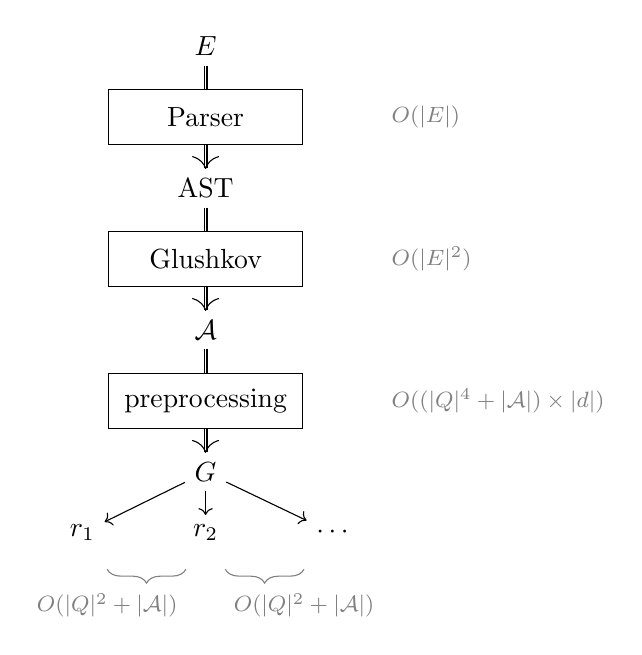
\begin{tikzpicture}[
        block/.style={%
          draw,
          fill=white,
          rectangle,
          minimum height=7mm,
          minimum width={width("preprocessing")+4mm}
        }
      ]

        \node        (regex)                              {$E$};

        \onslide<2->{
          \node[block] (parser)    [below=3mm of regex]      {Parser};
          \node        (ast)       [below=3mm of parser]        {AST};

          \draw[double]     (regex)  -- (parser);
          \draw[double, ->] (parser) -- (ast);

          \node[text=gray] [right=of parser] {\footnotesize $O(|E|)$};
        }

        \onslide<3->{
          \node[block] (glushkov)  [below=3mm of ast]       {Glushkov};
          \node        (automaton) [below=3mm of glushkov]  {$\mathcal{A}$};

          \draw[double]     (ast)      -- (glushkov);
          \draw[double, ->] (glushkov) -- (automaton);

          \node[text=gray] [right=of glushkov] {\footnotesize $O(|E|^2)$};
        }

        \onslide<4->{
          \node[block] (preproc)   [below=3mm of automaton] {preprocessing};
          \node        (dag)       [below=3mm of preproc]   {$G$};

          \draw[double]     (automaton) -- (preproc);
          \draw[double, ->] (preproc)   -- (dag);

          \node[text=gray] [right=of preproc]
            {\footnotesize $O((|Q|^4 + |\mathcal{A}|) \times |d|)$};
        }

        \onslide<5->{
          \node        (out2)      [below=3mm of dag]       {$r_2$};
          \node        (out1)      [left=of out2]           {$r_1$};
          \node        (out3)      [right=of out2]          {$\cdots$};

          \path[->]
            (dag) edge node {} (out1)
            (dag) edge node {} (out2)
            (dag) edge node {} (out3);

          \draw
            [gray,decorate,decoration={brace,amplitude=5pt,mirror,raise=4pt},yshift=0pt]
            (-1.25, -6.5) -- (-0.25, -6.5) node
            [gray,midway,yshift=-0.6cm,xshift=-5mm,text=gray]
            {\footnotesize $O(|Q|^2 + |\mathcal{A}|)$};
          \draw
            [gray,decorate,decoration={brace,amplitude=5pt,mirror,raise=4pt},yshift=0pt]
            (0.25, -6.5) -- (1.25, -6.5) node
            [gray,midway,yshift=-0.6cm,xshift=5mm,text=gray]
            {\footnotesize $O(|Q|^2 + |\mathcal{A}|)$};
        }
      \end{tikzpicture}
    \end{center}
    % add scheme of implem details
  \end{frame}

  \begin{frame}[fragile]{Implementation (2)}
    \begin{columns}
      \begin{column}{0.55\textwidth}
        On GitHub
        \begin{itemize}
           \item \textbf{\href{https://github.com/remi-dupre/enum-spanner}{remi-dupre/enum-spanner}}
          \item
            \textbf{\href{https://github.com/remi-dupre/enum-spanner-rs}{remi-dupre/enum-spanner-rs}}
        \end{itemize}

        \vspace{2cm}

        \tiny
        \begin{minted}{bash}
>> echo "read [link1](perdu.com) or [link2](qwant.com)" |
   ./enum "\[(?P<text>([^\]]*))\]\((?P<url>[^\)]*)\)"

1 - match:"[link1](perdu.com)" text:"link1" url:"perdu.com"
2 - match:"[link2](qwant.com)" text:"link2" url:"qwant.com"
        \end{minted}
      \end{column}
      \begin{column}{0.45\textwidth}
        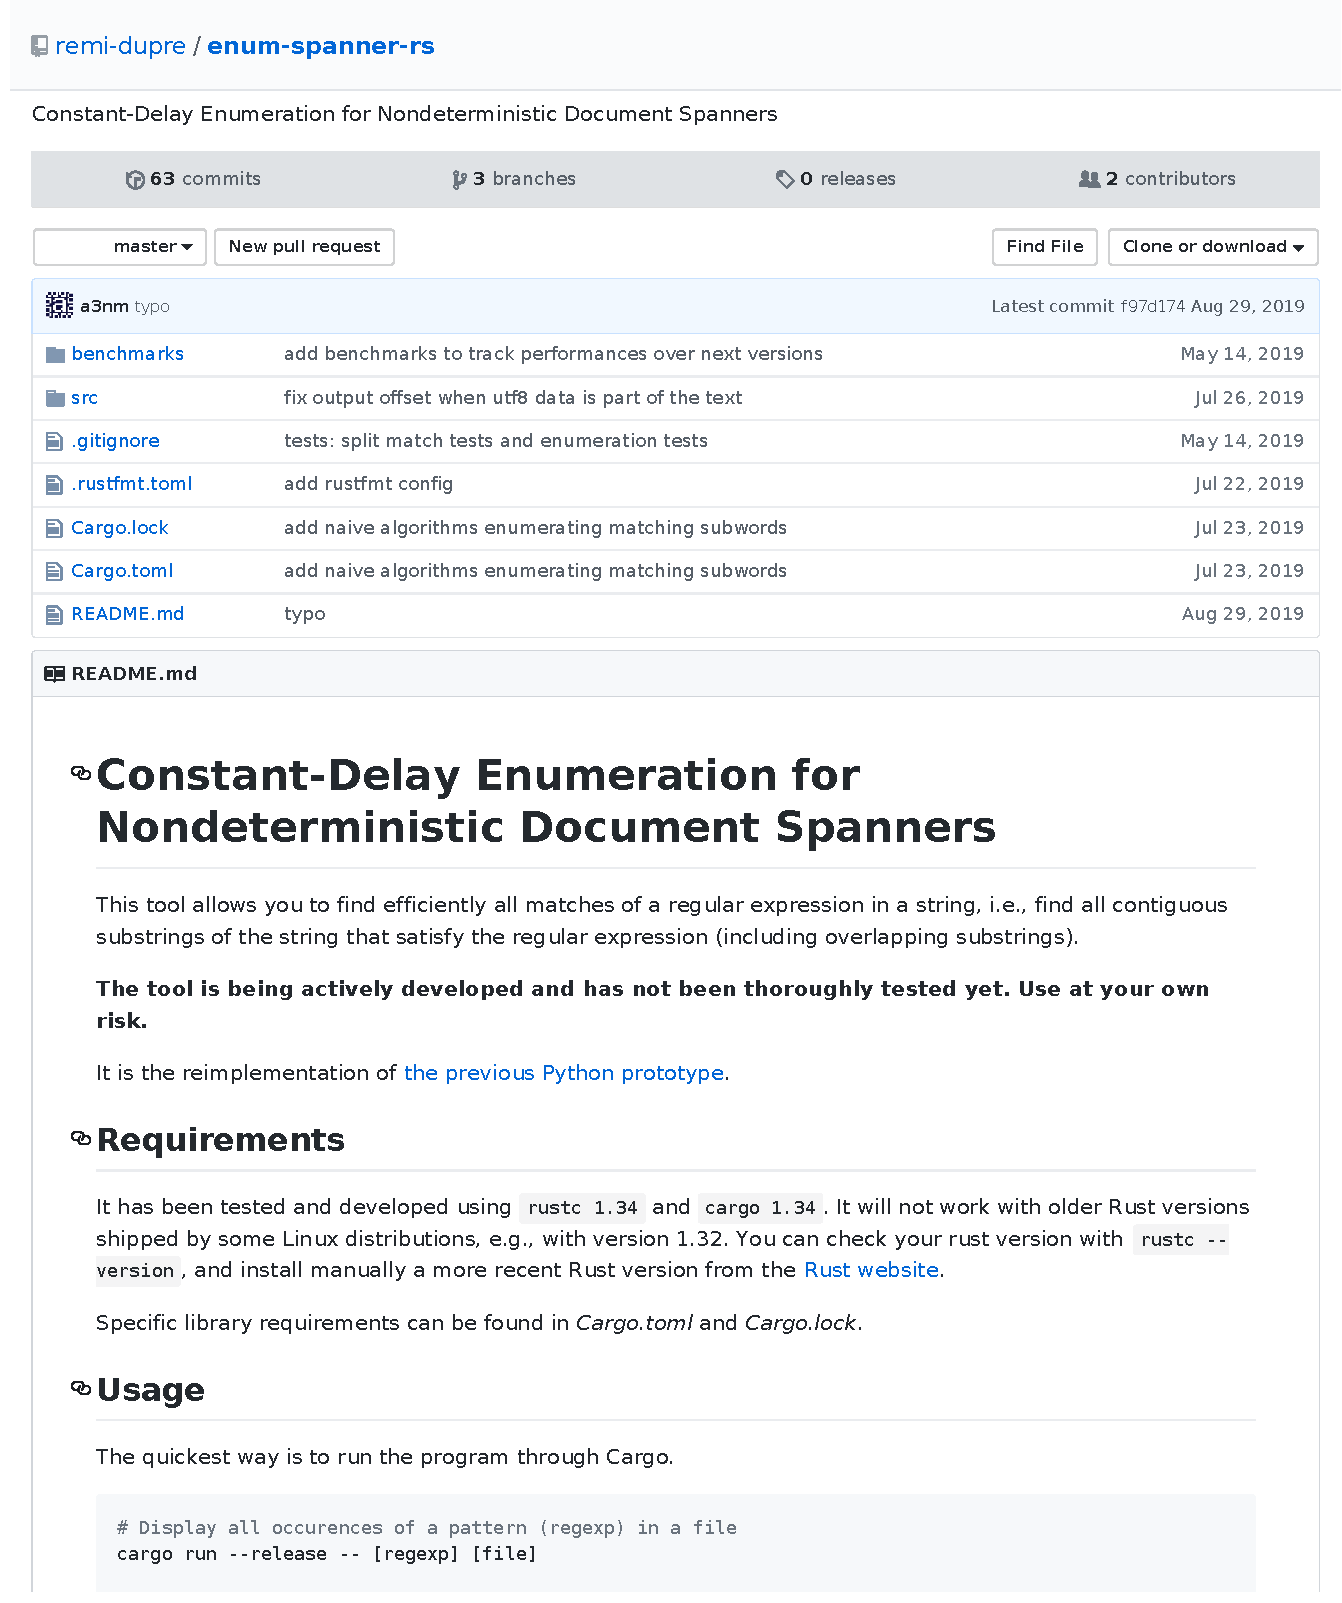
\includegraphics[width=5.5cm]{figures/github}
      \end{column}
    \end{columns}
  \end{frame}

  \begin{frame}{Competitors}
    \begin{itemize}
      \item  F. Florenzano, C. Riveros, M. Ugarte, S. Vansummeren, D. Vrgoc,
        \emph{Constant Delay Algorithms for Regular Document Spanners}, 2018
        (GitHub:
        \href{https://github.com/crivero1/SpannersConst}{crivero1/SpannersConst})
      \item Naive algorithms
    \end{itemize}

    \vfill

    \onslide<2->{
    Partial results:
      \begin{itemize}
        \item grep
        \item ripgrep
      \end{itemize}
    }
  \end{frame}

  \begin{frame}{Results (1)}
    \begin{figure}%
      % \caption{
      %   Enumeration speed of the different algorithms, over 10MB of DNA
      % }
      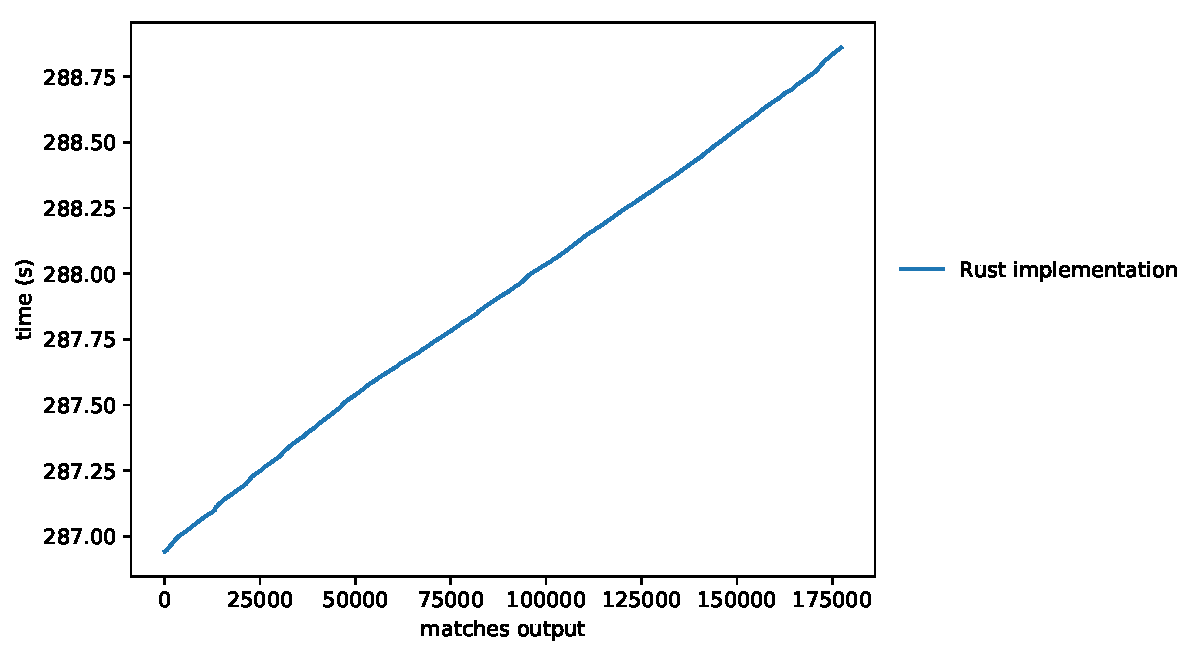
\includegraphics[trim={0 0 0 1.2cm}, clip, width=11cm]{figures/bench_enum_only}
    \end{figure}
  \end{frame}

  \begin{frame}{Results (2)}
    \only<1>{
      \begin{figure}%
        % \caption{
        %   Enumeration speed of the different algorithms, over 10MB of DNA
        % }
        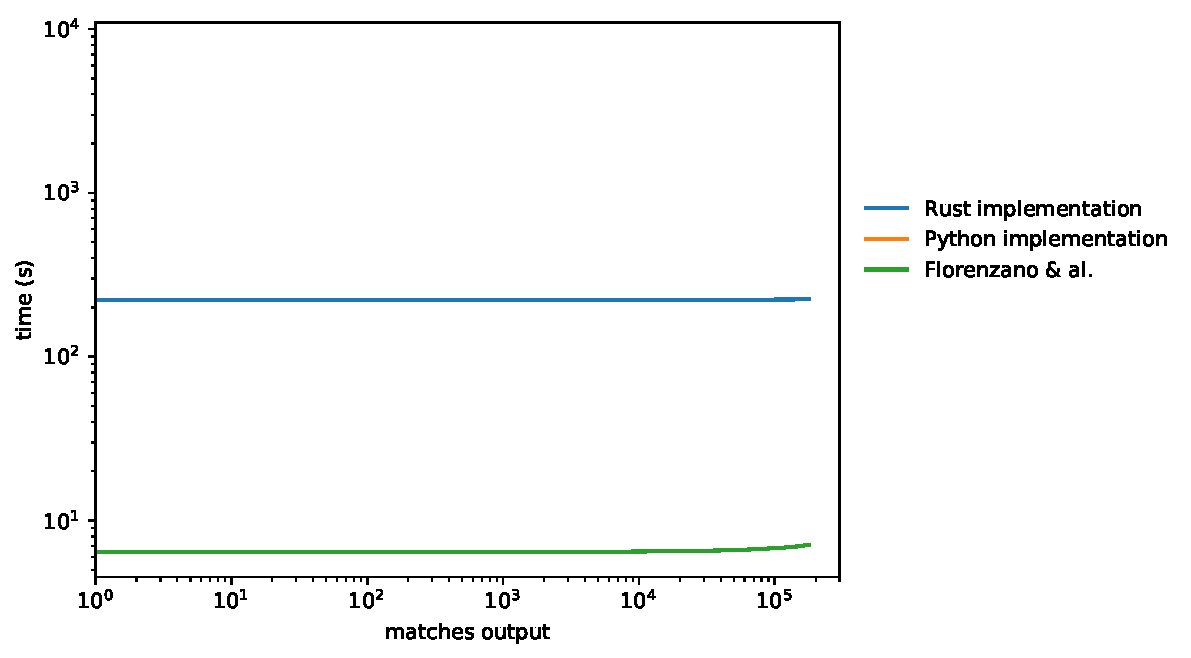
\includegraphics[trim={0 0 0 0}, clip, width=11cm]{figures/bench1}
      \end{figure}
    }
    \only<2>{
      \begin{figure}%
        % \caption{
        %   Enumeration speed of the different algorithms, over 10MB of DNA
        % }
        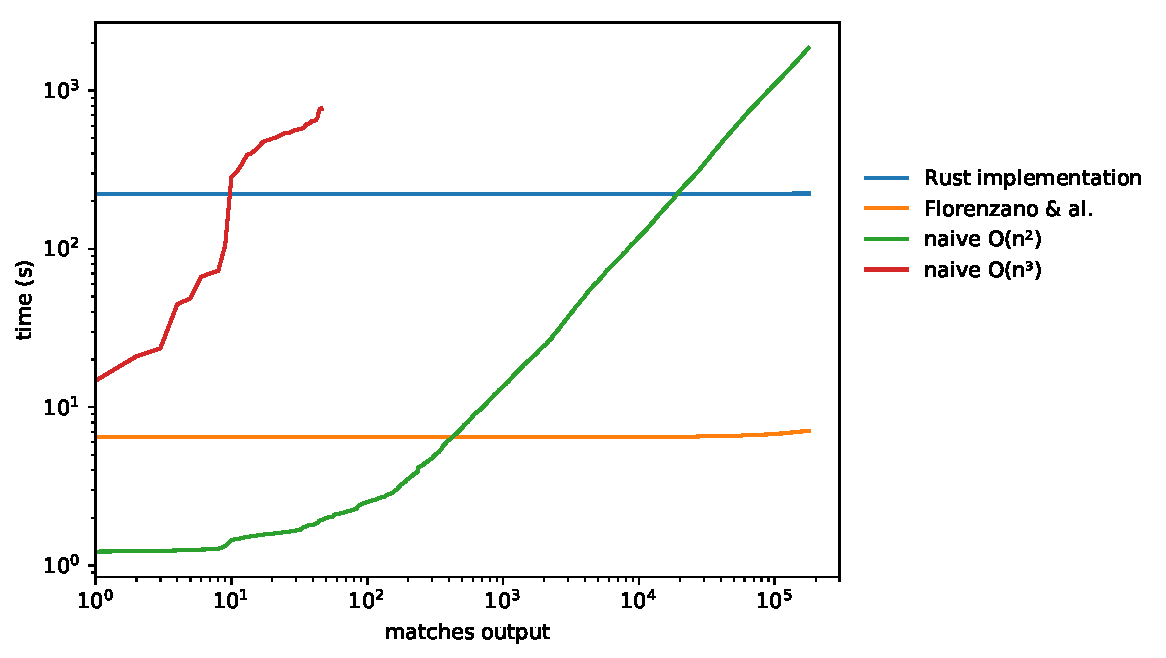
\includegraphics[trim={0 0 0 0}, clip, width=11cm]{figures/bench2}
      \end{figure}
    }
    \only<3>{
      \begin{figure}%
        % \caption{
        %   Enumeration speed of the different algorithms, over 10MB of DNA
        % }
        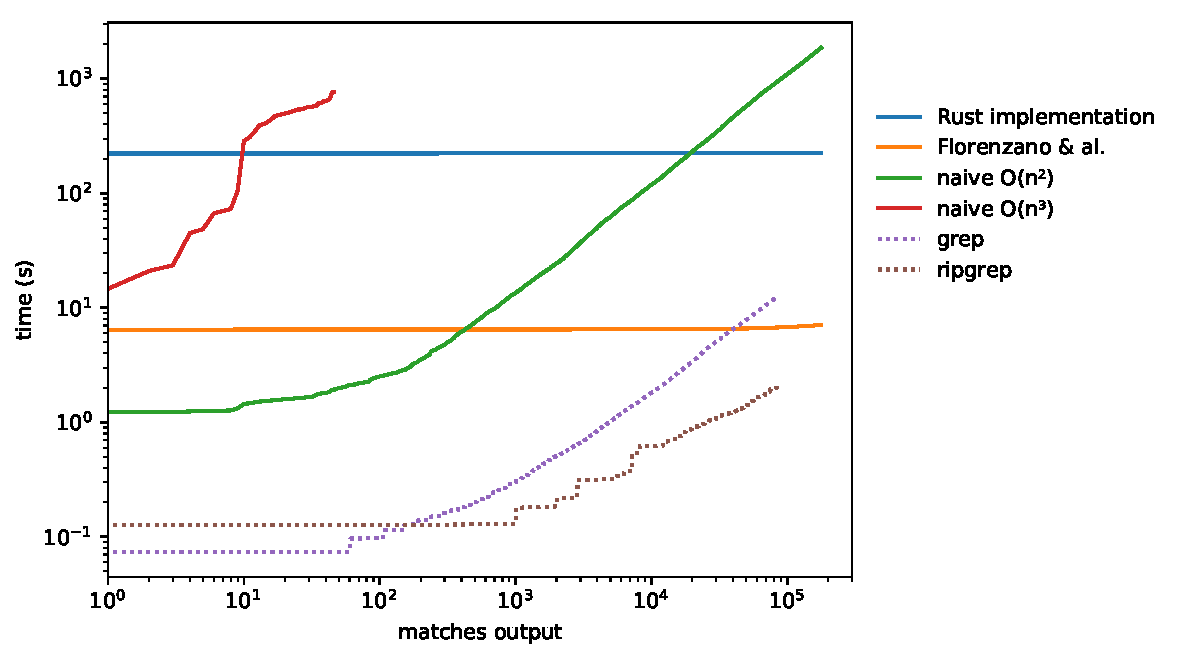
\includegraphics[trim={0 0 0 0}, clip, width=11cm]{figures/bench3}
      \end{figure}
    }
  \end{frame}


\section*{}

  \begin{frame}{}
    % \vspace{2cm}

    \begin{center}
      \Huge Conclusion
    \end{center}

    % Further work
    % \begin{itemize}
    %   \item early enumeration
    %   \item parallelization
    % \end{itemize}
  \end{frame}

\end{document}
